%iffalse
\let\negmedspace\undefined
\let\negthickspace\undefined
\documentclass[journal,12pt,onecolumn]{IEEEtran}
\usepackage{cite}
\usepackage{amsmath,amssymb,amsfonts,amsthm}
\usepackage{algorithmic}
\usepackage{graphicx}
\usepackage{textcomp}
\usepackage{xcolor}
\usepackage{txfonts}
\usepackage{listings}
\usepackage{enumitem}
\usepackage{mathtools}
\usepackage{pgfplots}
\usepackage{gensymb}
\usepackage{comment}
\usepackage[breaklinks=true]{hyperref}
\usepackage{tkz-euclide} 
\usepackage{listings}
\usepackage{gvv}                                        
%\def\inputGnumericTable{}                                 
\usepackage[latin1]{inputenc}                                
\usepackage{color}                                            
\usepackage{array}                                            
\usepackage{longtable}                                       
\usepackage{calc}                                             
\usepackage{multirow}                                         
\usepackage{hhline}                                           
\usepackage{ifthen}                                           
\usepackage{lscape}
\usepackage{tabularx}
\usepackage{array}
\usepackage{float}

\usepackage{enumitem}
\usepackage{xcolor}
%\usepackage{multicol}


\newtheorem{theorem}{Theorem}[section]
\newtheorem{problem}{Problem}
\newtheorem{proposition}{Proposition}[section]
\newtheorem{lemma}{Lemma}[section]
\newtheorem{corollary}[theorem]{Corollary}
\newtheorem{example}{Example}[section]
\newtheorem{definition}[problem]{Definition}
\newcommand{\BEQA}{\begin{eqnarray}}
\newcommand{\EEQA}{\end{eqnarray}}
\newcommand{\define}{\stackrel{\triangle}{=}}
\theoremstyle{remark}
\newtheorem{rem}{Remark}

\title{2011-ME-53-65}
\author{AI24BTECH11023 - Tarun Reddy Pakala}
\begin{document}
\bibliographystyle{IEEEtran}

\maketitle
\bigskip
\renewcommand{\thefigure}{\theenumi}
\renewcommand{\thetable}{\theenumi}
\begin{enumerate} [start=53]
\item The maximum deflection of the beam
\begin{enumerate}
    \item $\frac{24Pl^3}{Ebt^3}$
    \item $\frac{12Pl^3}{Ebt^3}$
    \item $\frac{8Pl^3}{Ebt^3}$
    \item $\frac{6Pl^3}{Ebt^3}$
\end{enumerate}
\subsection*{\textbf{Statement for Linked Answer Questions 54 and 55:}}
The temperature and pressure of air in a large reservoir are 400 K and 3 bar respectively. A converging- diverging nozzle of exit area $0.005 m^2$ is fitted to the wall of the reservoir as shown in the figure. The static pressure of air at the exit section for isentropic flow through the nozzle is 50 kPa. The characteristic gas constant and the ratio of specific heats of air are 0.287 kJ/kgK and 1.4 respectively.
%input command for figure1
		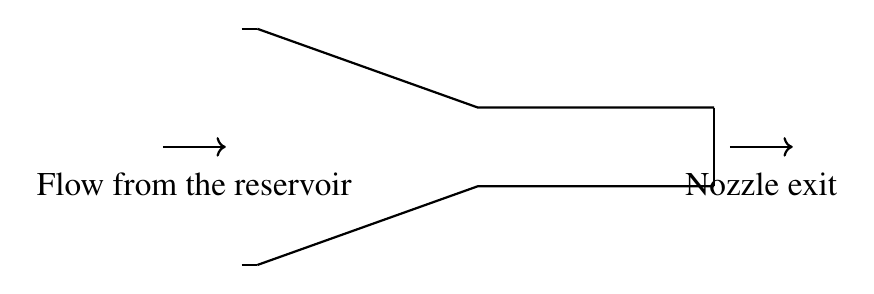
\begin{tikzpicture}
    % Draw the nozzle shape with short vertical lines at the opening
    \draw[thick] (-3,1.5) -- (-2.8,1.5);
    \draw[thick] (-3,-1.5) -- (-2.8,-1.5);
    \draw[thick] (-2.8,1.5) -- (0,0.5) -- (3,0.5);
    \draw[thick] (-2.8,-1.5) -- (0,-0.5) -- (3,-0.5);
    
    % Vertical line at the nozzle exit
    \draw[thick] (3,0.5) -- (3,-0.5);

    % Flow direction arrows
    \draw[->, thick] (-4,0) -- (-3.2,0);
    \draw[->, thick] (3.2,0) -- (4,0);

    % Labels for the flow and nozzle exit, placed below arrows
    \node[below] at (-3.6,-0.2) {\large Flow from the reservoir};
    \node[below] at (3.6,-0.2) {\large Nozzle exit};
\end{tikzpicture}

\item The density of air in $kg/m^3$ at the nozzle exit is 
\begin{enumerate}
    \item 0.560
    \item 0.600
    \item 0.727
    \item 0.800
\end{enumerate}
\item The mass flow rate of air through the nozzle in $kg/s$ is
\begin{enumerate}
    \item 1.30
    \item 1.77
    \item 1.85
    \item 2.06
\end{enumerate}
\subsection*{\textbf{General Aptitude (GA) Questions}}
\subsection*{\textbf{Q.56-Q.60 carry one mark each.}}
\item Choose the word from the options given below that is most nearly opposite in meaning to the given word:\\ \textbf{Amalgamate} 
\begin{enumerate}
    \item merge
    \item split
    \item collect
    \item separate
\end{enumerate}
\item Which of the following option is the closest in the meaning to the word below: \\ \textbf{Inexplicable}
\begin{enumerate}
    \item Incomprehensible
    \item Indelible
    \item Inextricable
    \item Infallible
\end{enumerate}
\item If Log (P) = (1/2)Log (Q) = (1/3) Log (R), then which of the following options is TRUE?
\begin{enumerate}
    \item $\text{P}^2=\text{Q}^3\text{R}^2$
    \item $\text{Q}^2=\text{PR}$
    \item $\text{Q}^2=\text{R}^3\text{P}$
    \item $\text{R}=\text{P}^2\text{Q}^2$
\end{enumerate}
\item Choose the most appropriate word(s) from the options given below to complete the following sentence.\\
\textbf{I contemplated \underline{\hspace{3cm}} Singapore for my vacation but decided against it.}
\begin{enumerate}
    \item to visit
    \item having to visit
    \item visiting
    \item for a visit
\end{enumerate}
\item Choose the most appropriate word from the options given below to complete the following sentence. \\
\textbf{If you are trying to make a strong impression on your audience, you cannot do so by being understated, tentative or \underline{\hspace{3cm}}.}
\begin{enumerate}
    \item hyperbolic
    \item restrained
    \item argumentative
    \item indifferent
\end{enumerate}
\subsection*{\textbf{Q.61 to Q.65 carry two marks each.}}
\item A container originally contains 10 liters of pure spirit. From this container 1 liter of spirit is replaced with 1 liter of water. Subsequently, 1 liter of the mixture is again replaced with 1 liter of water and this process is repeated one more time. How much spirit is now left in the container?
\begin{enumerate}
    \item 7.58 liters
    \item 7.84 liters
    \item 7 liters
    \item 7.29 liters
\end{enumerate}
\item \textbf{Few school curricula include a unit on how to deal with bereavement and grief, and yet all students at some point in their lives suffer from losses through death and parting.} \\ Based on the above passage which topic would not be included in a unit on bereavement?
\begin{enumerate}
    \item how to write a letter of condolence
    \item what emotional stages are passed through in the healing process
    \item what the leading causes of death are
    \item how to give support to a grieving friend
\end{enumerate}
\item  P, Q, R and S are four types of dangerous microbes recently found in a human habitat. The area of each circle with its diameter printed in brackets represents the growth of a single microbe surviving human immunity system within 24 hours of entering the body. The danger to human beings varies proportionately with the toxicity, potency and growth attributed to a microbe shown in the figure below.
%input command for figure 2
	\begin{figure}[!ht]
\centering
\resizebox{3cm}{3cm}{%
\begin{circuitikz}
\tikzstyle{every node}=[font=\LARGE]
\draw [ line width=0.6pt](2.75,12) to[sinusoidal voltage source, sources/symbol/rotate=auto] (3.25,11.5);
\draw [ line width=0.6pt](3.25,11.75) to[european resistor] (9.5,11.75);
\draw [line width=0.6pt, ->, >=Stealth] (9.5,11.75) -- (9.5,11);
\draw [ line width=0.6pt](4,12.25) to[short] (4,11.25);
\draw [ line width=0.6pt](4,11.5) to[short] (4,11);
\draw [ line width=0.6pt](8.75,12.25) to[short] (8.75,11);
\draw [ line width=0.6pt](4,11.25) to[short] (4.5,11.25);
\draw [ line width=0.6pt](8.75,11.25) to[short] (8.25,11.25);
\draw [ line width=0.6pt](4.25,11.25) to[short] (5.25,11.25);
\draw [ line width=0.6pt](8.25,11.25) to[short] (7.25,11.25);
\draw [ line width=0.6pt](5,11.25) to[european resistor] (5,8.5);
\draw [ line width=0.6pt](7.5,11.25) to[european resistor] (7.5,8.5);
\draw [ line width=0.6pt](4.75,8.5) to[short] (8,8.5);
\draw [line width=0.6pt, ->, >=Stealth] (6.25,8.5) -- (6.25,7.75);
\node [font=\normalsize] at (6.75,8) {Bus 3};
\node [font=\normalsize] at (4,12.5) {Bus 1};
\node [font=\normalsize] at (8.75,12.5) {Bus 2};
\node [font=\normalsize] at (6.25,12.25) {j q};
\node [font=\normalsize] at (4.5,10) {j r};
\node [font=\normalsize] at (8.25,9.75) {j p};
\end{circuitikz}
}%

\label{fig:my_label}
\end{figure}

\\
A pharmaceutical company is contemplating the developement of a vaccine against the most dangerous microbe. Which microbe should the company target in its first attempt?
\begin{enumerate}
    \item P
    \item Q
    \item R
    \item S
\end{enumerate}
\item The variable cost ({V}) of manufacturing a product varies according to the equation V= 4q, where q is the quantity produced. The fixed cost (F) of production of same product reduces with q according to the equation F = 100/q. How many units should be produced to minimize the total cost (V+F)?
\begin{enumerate}
    \item 5
    \item 4
    \item 7
    \item 6
\end{enumerate}
\item  A transporter receives the same number of orders each day. Currently, he has some pending orders (backlog) to be shipped. If he uses 7 trucks, then at the end of the 4th day he can clear all the orders. Alternatively, if he uses only 3 trucks, then all the orders are cleared at the end of the 10th day. What is the minimum number of trucks required so that there will be no pending order at the end of the 5th day?
\begin{enumerate}
    \item 4
    \item 5
    \item 6
    \item 7
\end{enumerate}
\end{enumerate}
\end{document}
